Vous pouvez rechercher n'importe quelle chanson ou artiste disponibles sur ChromaCase.
\\\\
Afin d’accéder à la page de recherche, cliquez sur le bouton recherche se trouvant sur la gauche de la page principale (Voir Capture \ref{fig:access-search}).

\begin{figure}[H]
	\begin{subfigure}[b]{0.7\textwidth}
		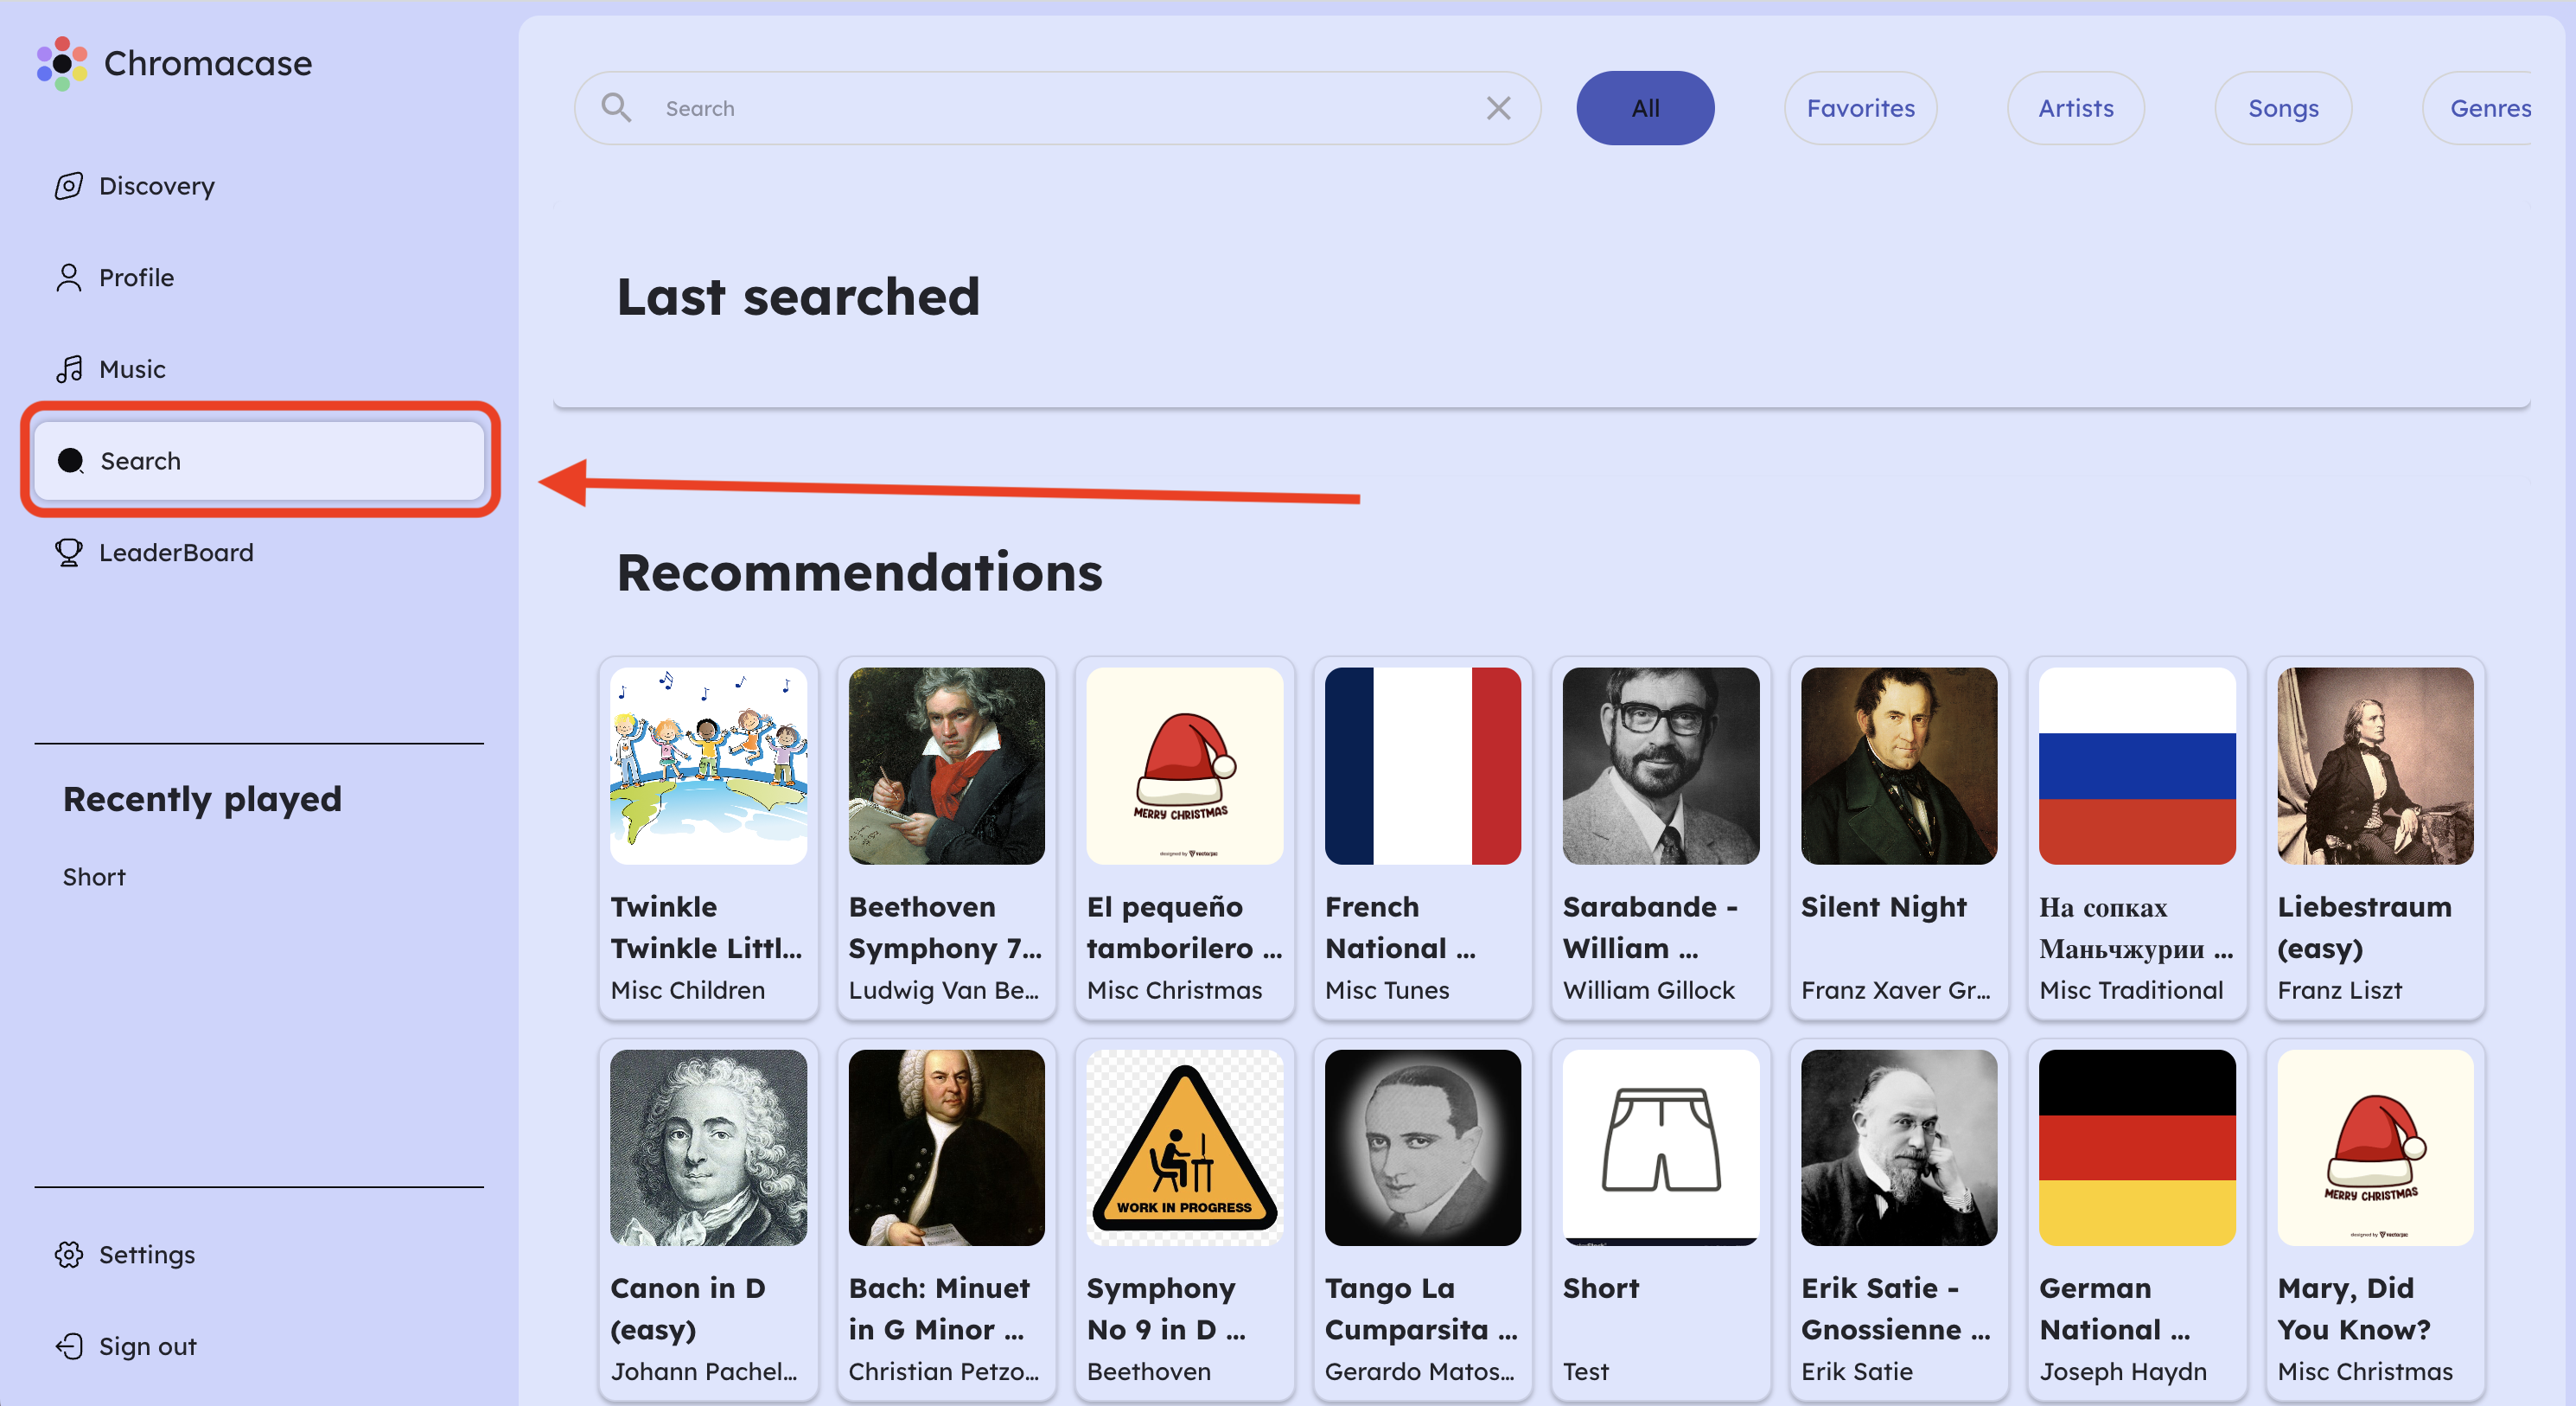
\includegraphics[width=\linewidth]{../\dir/guide/search/access-search.png}
		\caption{Version navigateur}
	\end{subfigure}
	\begin{subfigure}[b]{0.25\textwidth}
		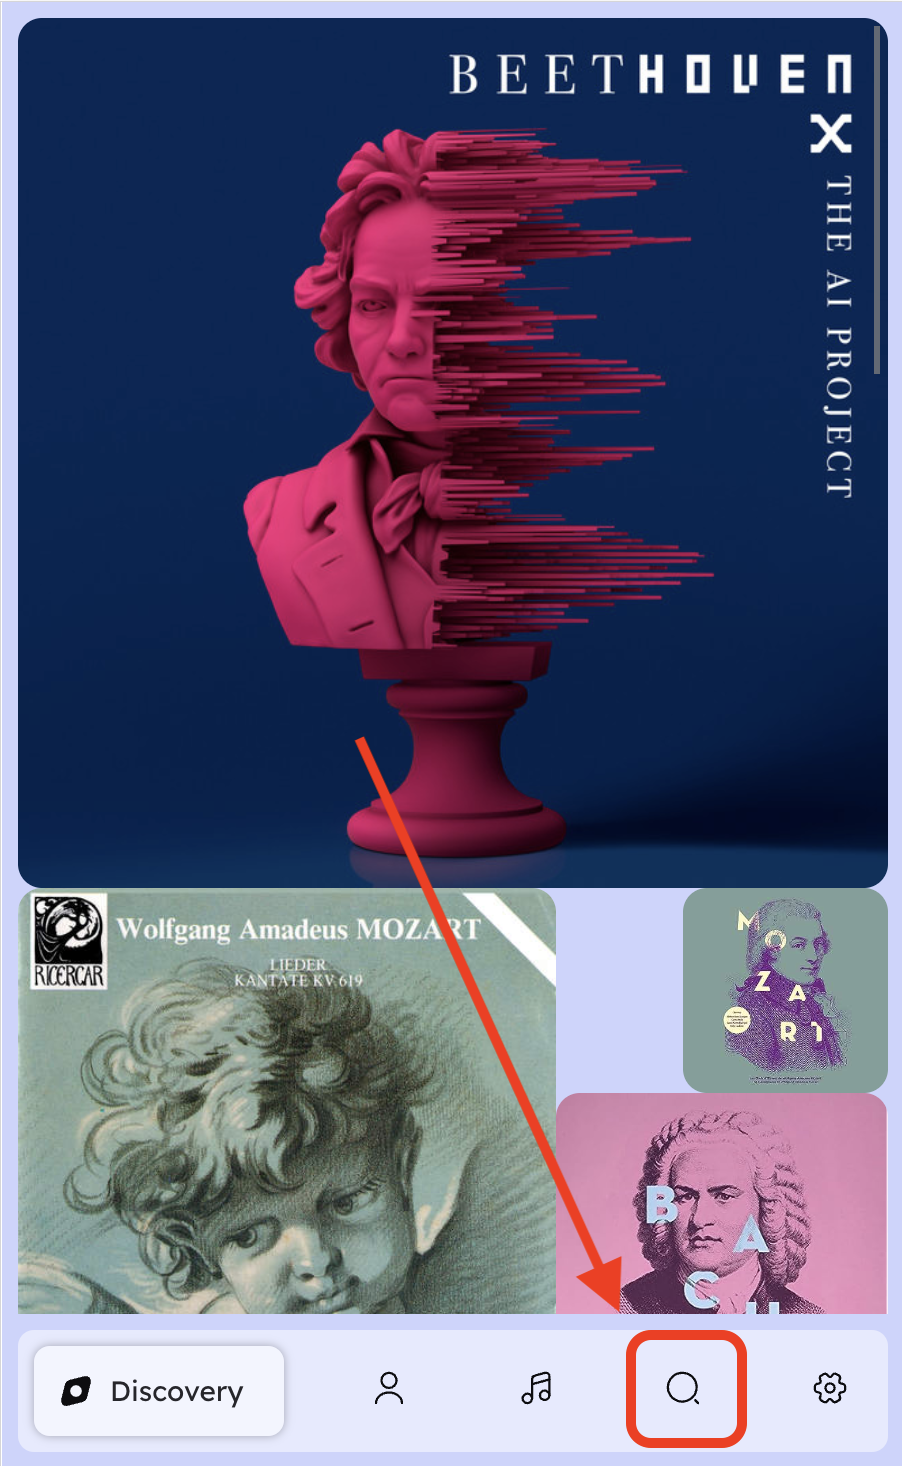
\includegraphics[width=\linewidth]{../\dir/guide/search/access-search-mobile.png}
		\caption{Version mobile}
	\end{subfigure}
	\caption{Accéder à la page de recherche}
	\label{fig:access-search}
\end{figure}
\begin{figure}[H]
	\begin{subfigure}[b]{0.7\textwidth}
		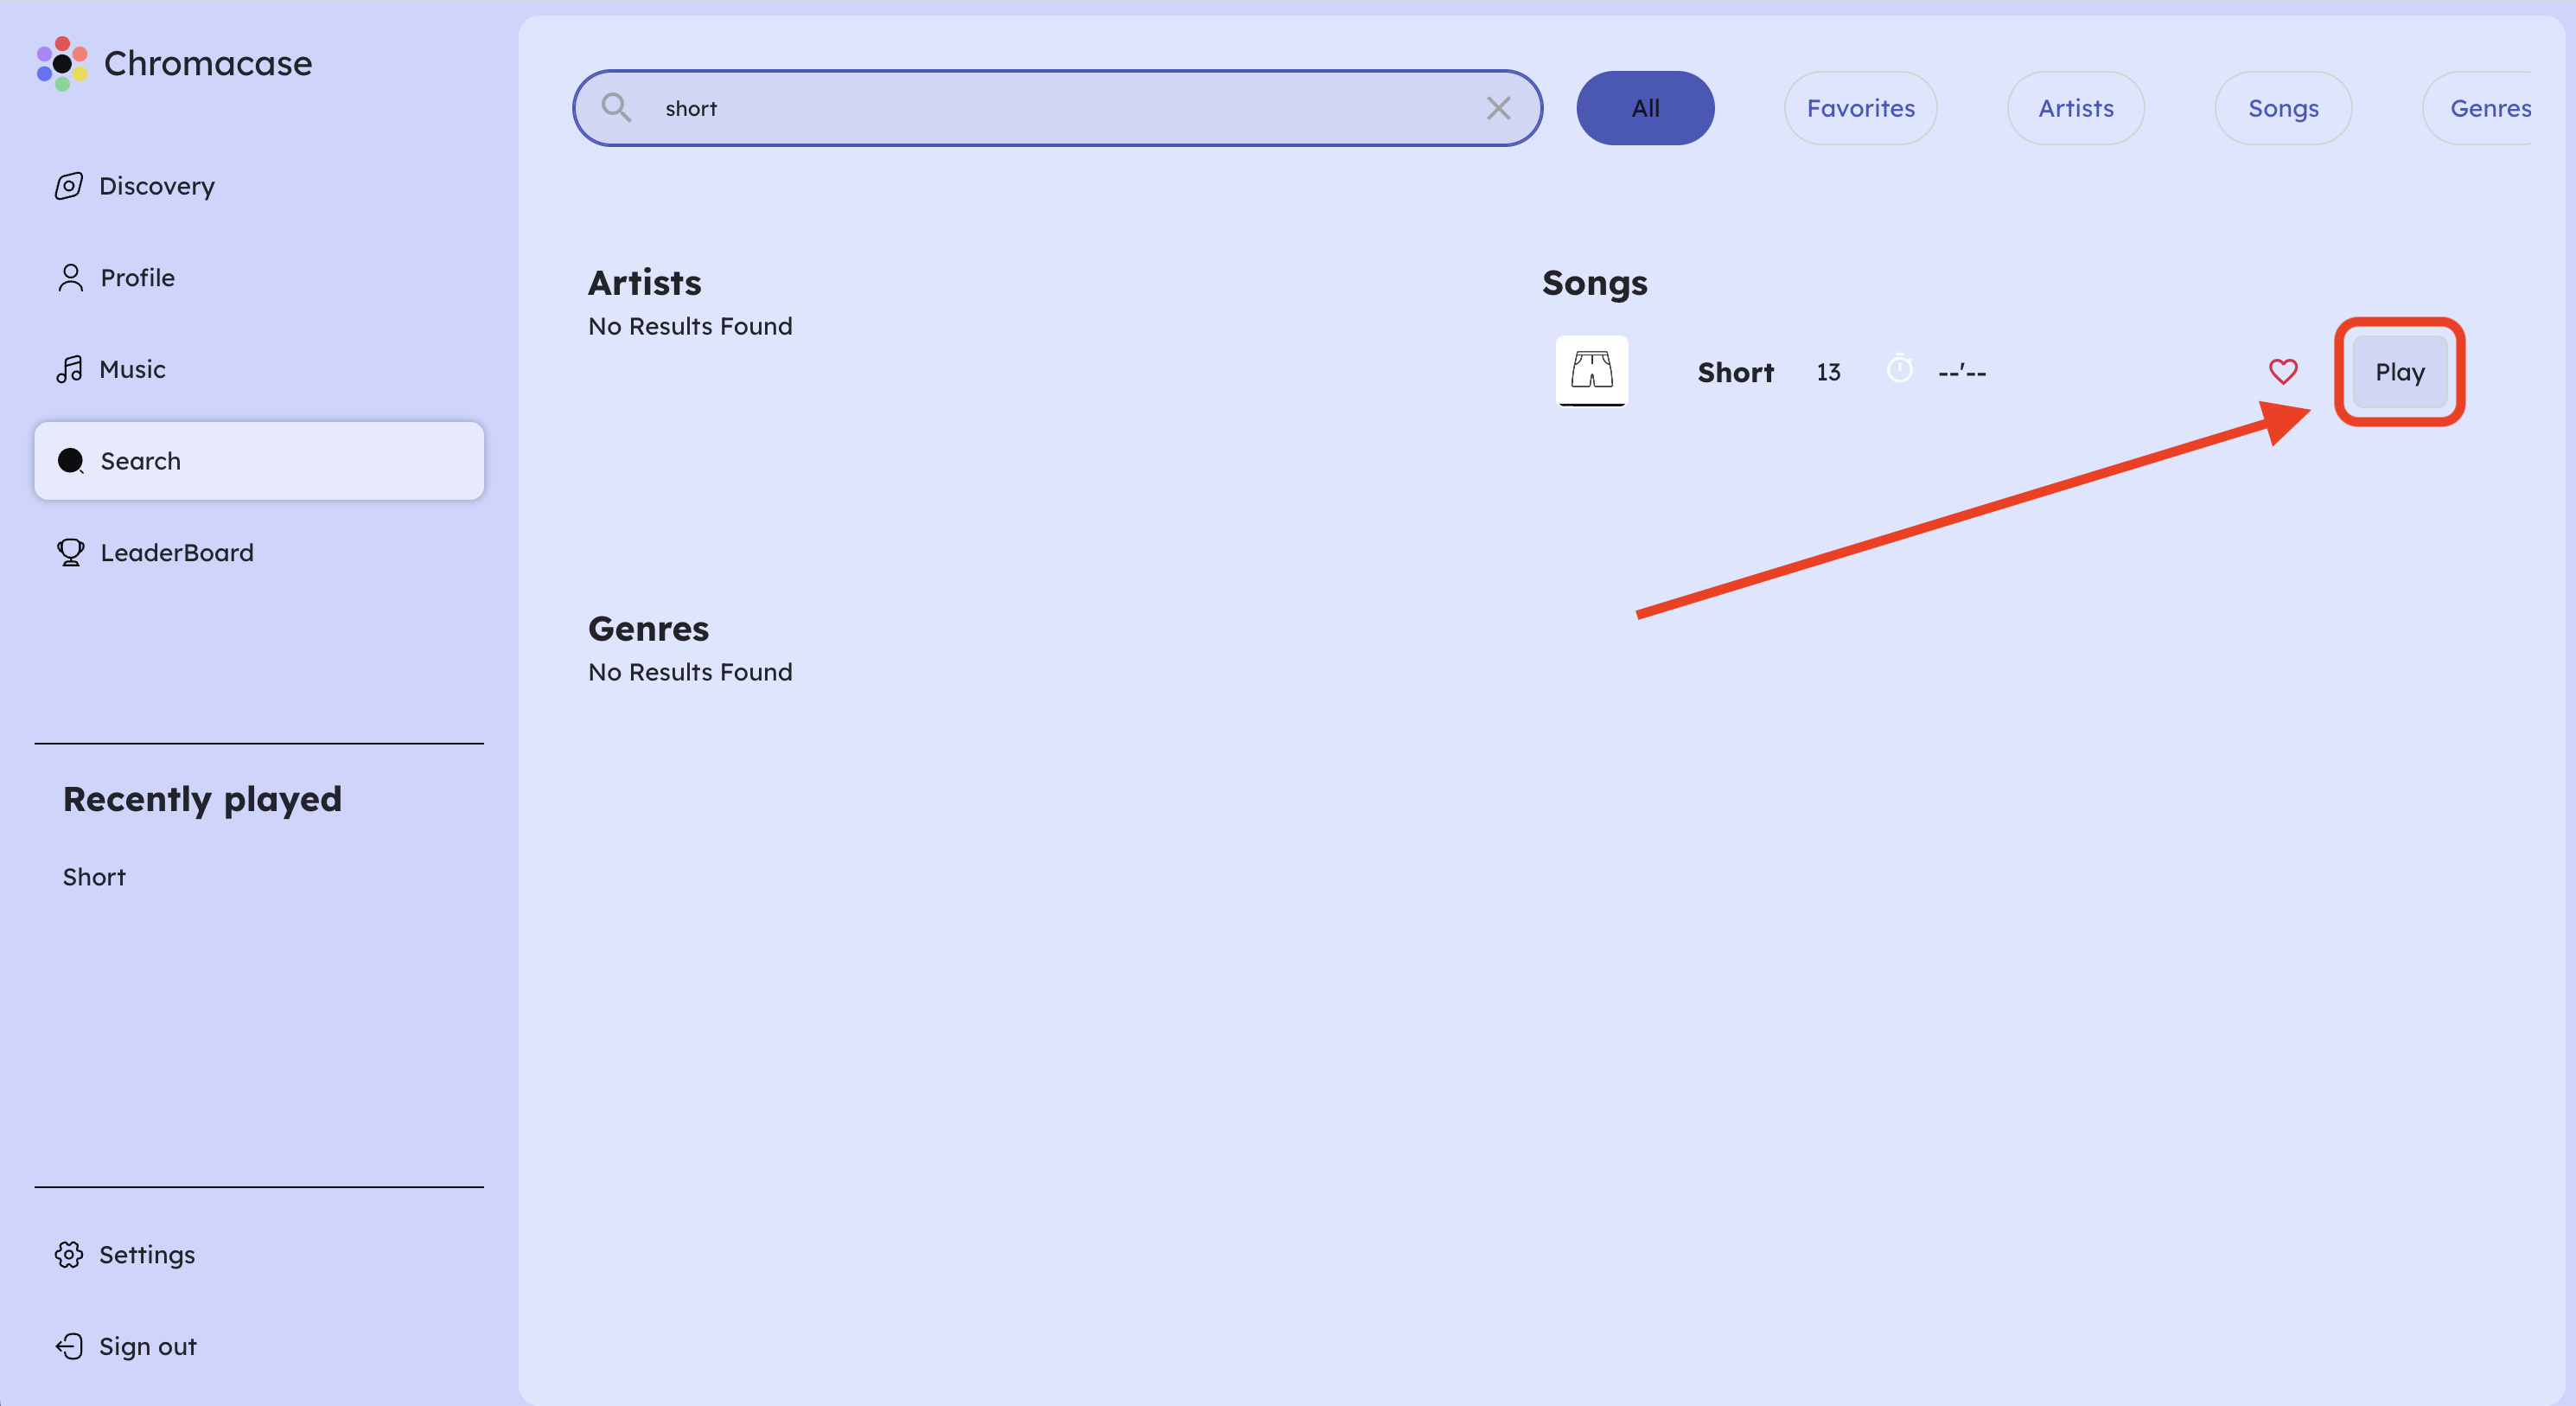
\includegraphics[width=\linewidth]{../\dir/guide/search/search.png}
		\caption{Version navigateur}
	\end{subfigure}
	\begin{subfigure}[b]{0.25\textwidth}
		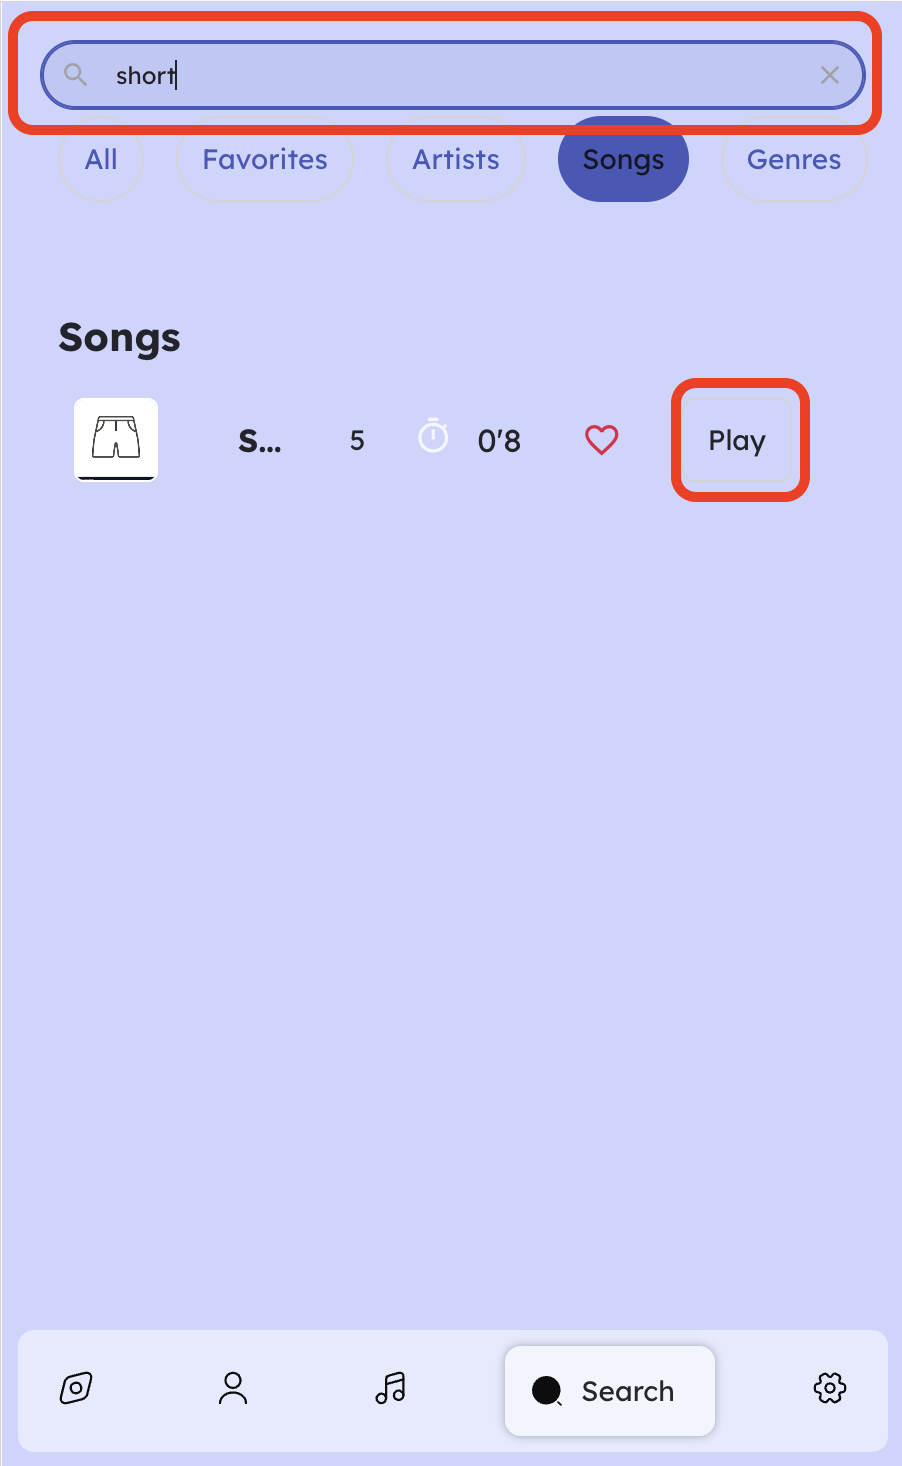
\includegraphics[width=\linewidth]{../\dir/guide/search/search-mobile.png}
		\caption{Version mobile}
	\end{subfigure}
	\caption{Page de recherche}
	\label{fig:search}
\end{figure}

\subsubsection{Rechercher une chanson}
Commencez à taper le nom de la chanson avec une catégorie compatible. Les catégories compatibles sont “Tout” et “Morceaux” (Voir Capture \ref{fig:search}).

\subsubsection{Rechercher un artiste}
Commencez à taper le nom de la chanson avec une catégorie compatible. Les catégories compatibles sont “Tout” et “Artistes” (Voir Capture \ref{fig:search}).